\documentclass[]{article}

\usepackage{xcolor}
\usepackage{amsmath}
\usepackage{amsthm}
\usepackage{amssymb}
\usepackage{esint}
\usepackage[parfill]{parskip}
\usepackage{hyperref}
\usepackage{floatrow}
\usepackage{graphicx}
\usepackage{multirow}
\usepackage{multicol}
\usepackage{listings}

\newtheorem{theorem}{Theorem}
\newtheorem{lemma}{Lemma}
\newtheorem{corollary}[theorem]{Corollary}
\newtheorem{proposition}{Proposition}[section]

\theoremstyle{remark}
\newtheorem*{remark}{Remark}
\newtheorem*{hint}{Hint}

\bibliographystyle{plainurl}

\newcounter{mycounter}

\lstnewenvironment{mylst}[2]{
    \lstset{
        numbers = left,
        breaklines = true,
        keywordstyle = \color{blue}\bfseries,
        numberstyle = \tiny\color{gray},
        commentstyle = \color{green!30!black},
        stringstyle = \color{violet},
        language = #1
    }
    \refstepcounter{mycounter}
    \begin{center}
        \textbf{\large{Listing \themycounter: #1}} \\
        \textbf{#2}
    \end{center}
}
{
    \vspace{2 em}
}


\title{Technical Typesetting Assignment}
\author{Atishay Jain}
\date{\today}

\begin{document}
\maketitle
\tableofcontents
\newpage
\section{Listings and Environments}

\begin{mylst}{[LaTeX]TeX}{An Example}
\begin{lstlisting}
%A regular \lstlisting environment won't work. You'll have to use \lstnewenvironment to define a custom environment.
\end{lstlisting}
\end{mylst}

\begin{mylst}{Python}{Regular Stuff}
from scipy import *
#The custom environment you define should be numbered as well. We did this in our tutorial. Think about what arguments you can pass to it.
print("Hello!")
\end{mylst}

\begin{mylst}{C++}{Generic Title}
#include <iostream>
using namespace std;

//From the three examples, you must have observed what you can hardcode.

int main(int argc, char* argv[])
{
    cout<<"Hello!"<<endl;
}
\end{mylst}

The \texttt{2em} vertical space after the listing is part of the custom environment.

\newpage

\section{Formal Logic: Figures and Tables}

\begin{figure}[H]
    \centering
    \begin{floatrow}
    \ffigbox[0.4\textwidth]{\caption{Aristotle: The first formal logician}}{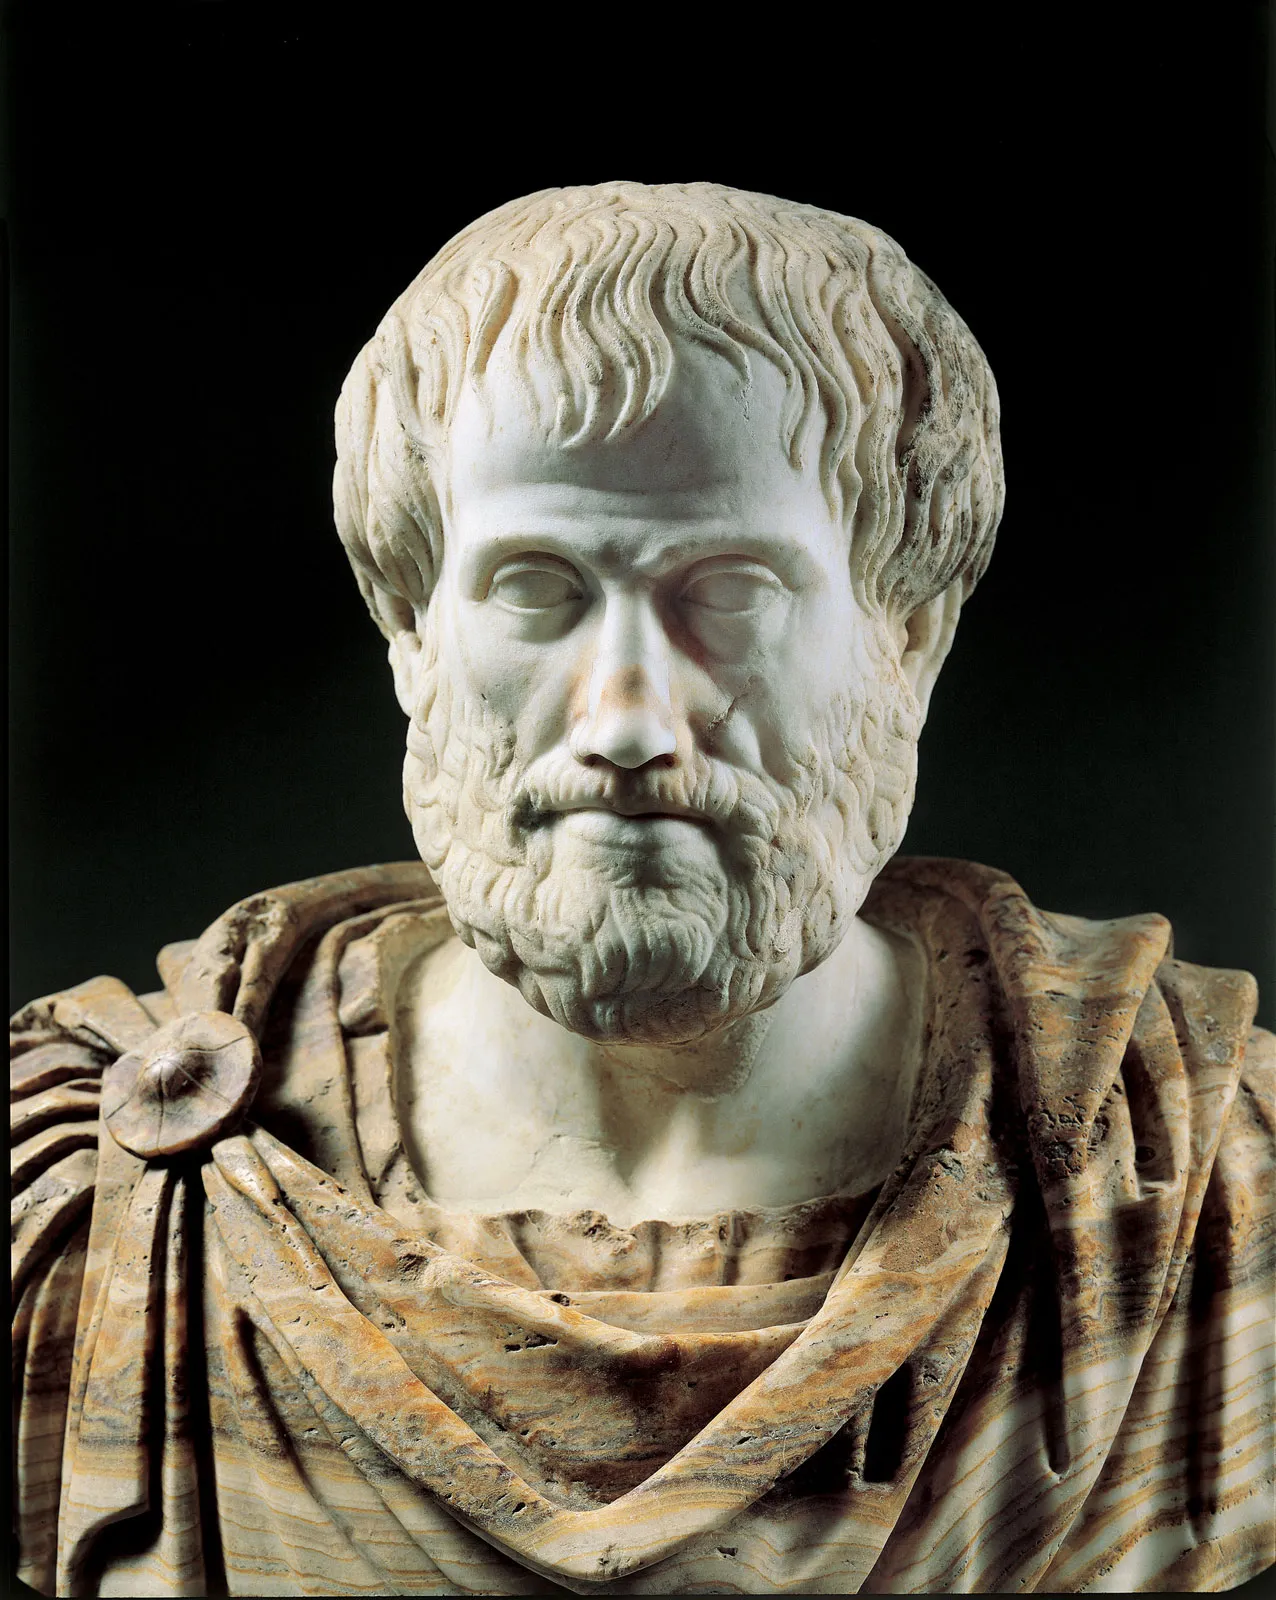
\includegraphics[width=0.4\textwidth]{Aristotle.png}}
    \ffigbox[0.525\textwidth]{\caption{\hspace{0.6 ex}Saul Kripke: \hspace{0.6 ex}we've  \hspace{0.6 ex} come \hspace{0.6 ex} a  long way since then.}}{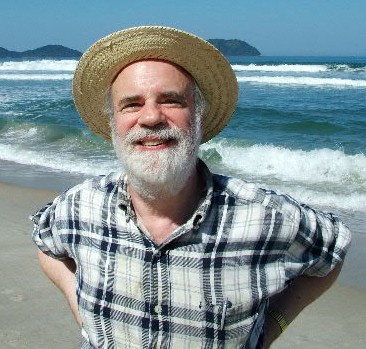
\includegraphics[width=0.525\textwidth]{Kripke.jpeg}}
    \end{floatrow}
\end{figure}

\href{https://www.britannica.com/biography/Aristotle#/media/1/34560/76426}{Aristotle image source} \\
\href{https://commons.wikimedia.org/w/index.php?curid=5763037}{Saul Kripke image source} \\
Make sure you follow these links, so you know where the hyperlinks lead to when you typeset it yourself.

\begin{table}[H]
    \centering
    \begin{tabular}{p{3.7 cm}|p{3.7 cm}}
         \hline
         \textbf{Assertion} & \textbf{Negation} \\
         \hline
         $p(x)$ & $\neg{p(x)}$ \\
         \hline
         \multirow{2}{*}{$\perp$} & $p(x) \vee \neg p(x)$ \\
         & $\top$ \\
         \hline
         \multirow{2}{*}{$p(x) \wedge q(x)$} & $\neg (p(x) \wedge q(x))$ \\ 
         & $\neg p(x) \vee \neg q(x)$ \\
         \hline
         $\exists x.p(x)$ & $\forall x. \neg p(x)$\\
         \hline
         \multirow{2}{*}{$p(x) \Rightarrow q(x)$} & $\neg (\neg p(x) \lor q(x))$ \\
         & $p(x) \land \neg q(x)$\\
         \hline
         \multicolumn{2}{c}{This statement is false.} \\
         \hline
    \end{tabular}
    \caption{Some First Order Logic, and an absurdity.}
    \label{tab:my_label}
\end{table}

This table uses multirow as well as multicolumn. Replicate it as well as you can.

\newpage

\section{Maths, Theorems and References}

\begin{theorem}[Divergence Theorem]
\begin{equation*}
    \iiint_V (\boldsymbol{\nabla} \cdot \mathbf{F}) dV = \oiint_S (\mathbf{F} \cdot \mathbf{\hat{n}}) dS
\end{equation*}
\end{theorem}

\begin{remark}
You have definitely studied and applied the theorem extensively in
MA 105. It also shows up as Gauss’ Law in electrodynamics.
\end{remark}

\begin{proposition}[Georg Cantor]
Let $\mathbb{N}$ be the set natural numbers. Denote its cardinality $|\mathbb{N}|$ by $\aleph_0$. Let $\mathbb{R}$ be the set of real numbers. Its cardinality $\mathfrak{c}$ is sometimes called the cardinality of the continuum. $\mathfrak{c} = 2^{\aleph_0}$ 
\end{proposition}

\begin{hint}
You will find the \texttt{$\backslash$ \hspace{-0.5 em}mathfrak} command useful to typeset the above.
\end{hint}

\begin{lemma}[Jordan Normal Form]\label{lemma1}
For every matrix M in $\mathbb{C}^{\kappa \times \kappa}$ having eigenvalues $\gamma_1, ..., \gamma_k$, with algebraic multiplicities $m_1, ..., m_k$ respectively, there is an invertible matrix P and a matrix D of the form D = Diag($J_1, ...,J_k$) with each block $J_i$ being a $m_i \times m_i$ matrix of the form

\vspace{-1 em}
\begin{equation*}
    J_i = 
    \begin{bmatrix} 
        \gamma_i & 1 & 0 & \dots & 0 \\
        0 & \gamma_i & 1 & \dots & 0 \\
        \vdots & \vdots & \vdots & \ddots & \vdots \\
        0 & 0 & 0 & \dots & 1 \\
        0 & 0 & 0 & \dots & \gamma_i \\
    \end{bmatrix}
\end{equation*}
\vspace{0.2 em}
and M = $P^{-1}DP$. Moreover, if M is an algebraic matrix, so are D and P, and their entries can be computed from the entries of M.
\end{lemma}

You have certainly studied that if M is defect free, that is, algebraic and multiplicities of its eigenvalues coincide, then it is similar to a diagonal matrix. If not, the Jordan Normal form is the next best thing. We cite \cite{ref1} for this lemma.

\begin{hint}
Look at the bibliography entry for this citation. It is a book. Specify the author, publisher, title, year and edition. Our bibliography style is
\texttt{plainurl}.
\end{hint}

Consider the last statement of Lemma \ref{lemma1}. (Yes, a cross reference.) Algebraic numbers are roots of polynomials with integer coefficients. They can be found efficiently. \cite{ref2}.

\begin{hint}
This citation is an article. Specify the author, year, title, journal, volume and number.
\end{hint}
\bibliography{assignment3}

\end{document}